\documentclass[11pt]{article}

% ---------- Packages ----------
\usepackage[utf8]{inputenc}
\usepackage[T1]{fontenc}
\usepackage{lmodern}
\usepackage[margin=1in]{geometry}
\usepackage{amsmath,amssymb}
\usepackage{siunitx}
\usepackage{graphicx}
\usepackage{float}
\usepackage{caption}
\usepackage{subcaption}
\usepackage{booktabs}
\usepackage{microtype}
\usepackage{fancyhdr}
\usepackage{xcolor}
\usepackage[colorlinks=true,linkcolor=blue!55!black,citecolor=blue!55!black,urlcolor=blue!55!black]{hyperref}

% ---------- Spacing / look ----------
\setlength{\parskip}{0.55em}
\setlength{\parindent}{0pt}
\captionsetup{font=small,labelfont=bf}
\graphicspath{{figures/}}

% ---------- Header / footer ----------
\pagestyle{fancy}
\fancyhf{}
\lhead{\small EE132 --- Automatic Control}
\rhead{\small Lab 6}
\cfoot{\thepage}
\renewcommand{\headrulewidth}{0.4pt}

% siunitx setup
\sisetup{detect-all,per-mode=symbol}

% ---------- Title ----------
\title{\vspace{-1.0cm}\textbf{Lab 6 Report}\\[0.3em]
\large Second-Order System Analysis of the Quanser QUBE-Servo\\ under Unity Feedback Control}
\author{Kaushik Vada \and Andrew Kong \and Aren Muniz \and Kai Ong}
\date{May 22, 2026}

\begin{document}
\maketitle
\thispagestyle{fancy}

% ---------- Abstract ----------
\begin{abstract}
\noindent This lab focused on analyzing the behavior of a second-order system using the
Quanser QUBE-Servo under unity feedback control. The experiment explored important
second-order system characteristics such as damping ratio, natural frequency, peak time,
and percent overshoot. A Simulink model was developed to implement unity feedback
position control, and a step input was applied to observe the servo response. The
experimental response was then compared with the theoretical calculations obtained from
the closed-loop transfer function. The results demonstrated the relationship between system
parameters and transient response behavior, while also reinforcing concepts related to
underdamped second-order systems and control system analysis.
\end{abstract}

% =====================================================================
\section{System Built}
% =====================================================================
The system built in this lab was a unity feedback position control system for the Quanser
QUBE-Servo. The setup consisted of the QUBE-Servo hardware connected to a Simulink
controller through QUARC. The Simulink model implemented a unity feedback loop where the
measured motor position was continuously compared to the desired reference position. The
model included a step input, summing junction, gain block, encoder feedback, and motor
voltage output. A \SI{1}{\radian} step input was applied at \SI{1}{\second}, and the
response was observed over a \SI{2.5}{\second} simulation interval.

\begin{figure}[H]
    \centering
    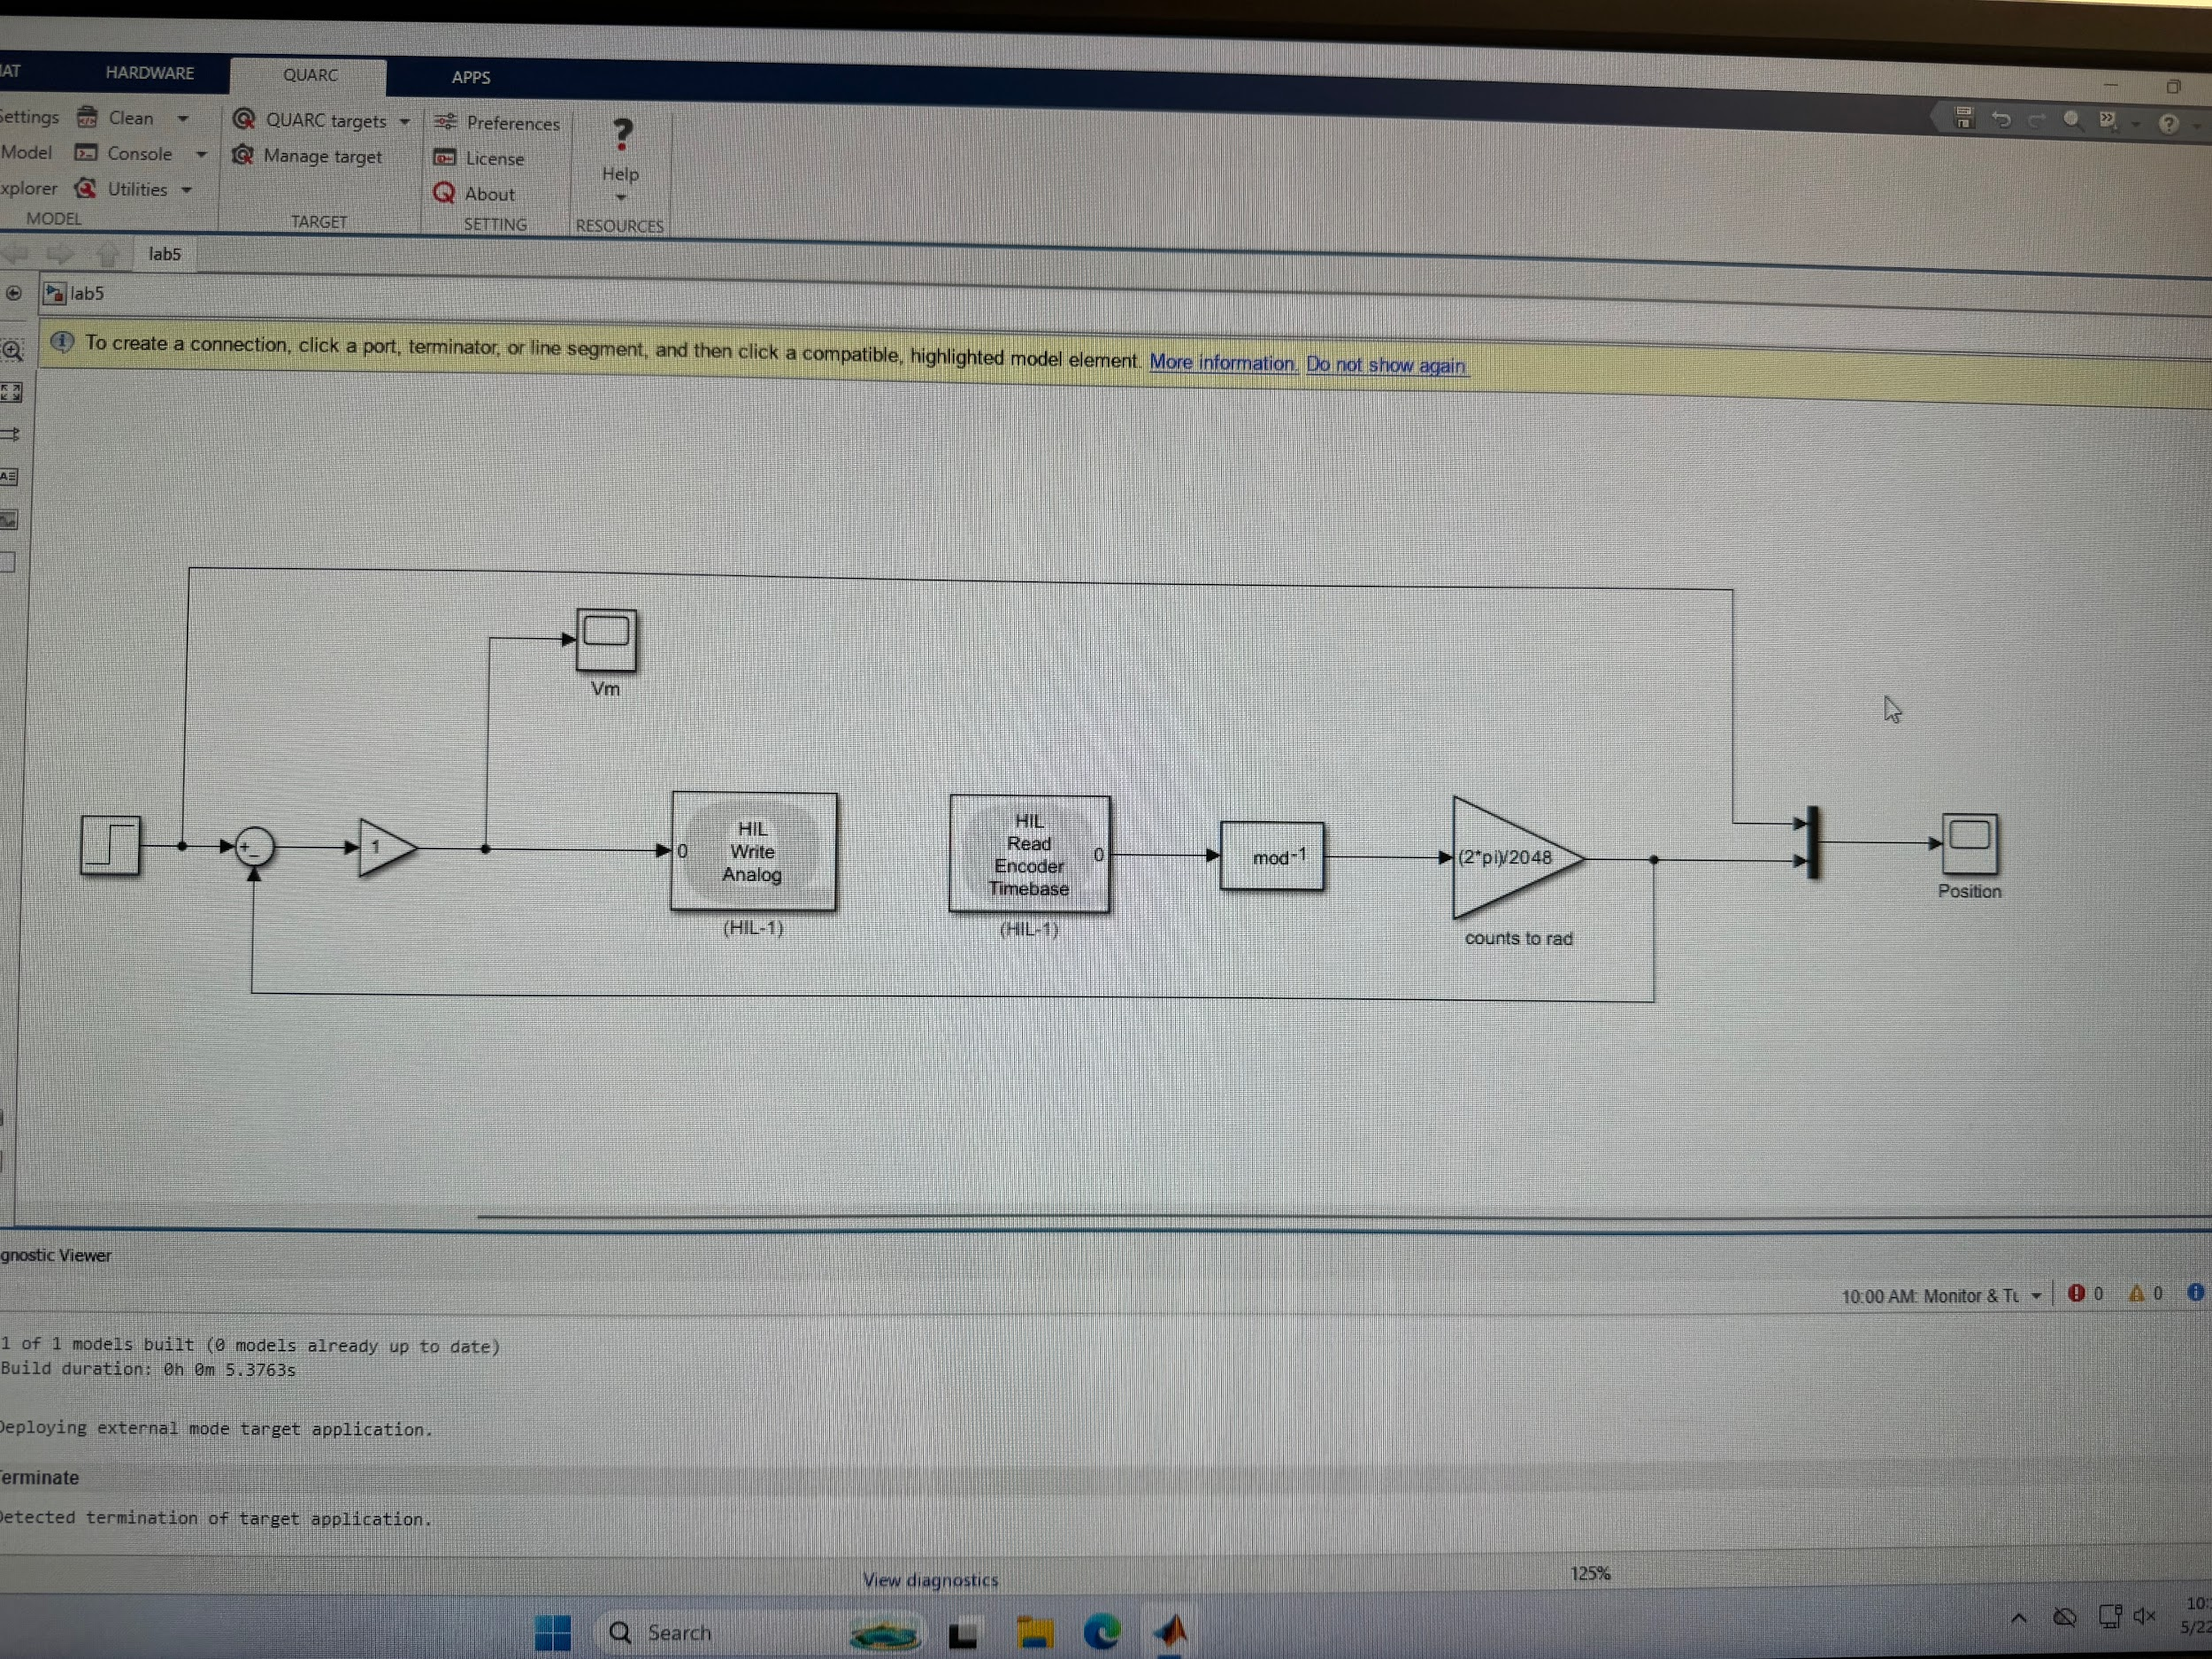
\includegraphics[width=0.95\textwidth]{model.jpg}
    \caption{QUARC/Simulink unity feedback position control model for the QUBE-Servo.
    The loop compares the encoder-measured position (converted from counts to radians)
    against the reference step and drives the motor through the HIL Write Analog block.}
    \label{fig:model}
\end{figure}

% =====================================================================
\section{In-Lab Exercises and Results}
% =====================================================================

\subsection{Natural Frequency and Damping Ratio}
Given the QUBE-Servo closed-loop equation under unity feedback (Equation~6 in the lab
manual) and the model parameters, the closed-loop response takes the standard second-order
form
\begin{equation}
    \frac{Y(s)}{R(s)} = \frac{\omega_n^{2}}{s^{2} + 2\zeta\omega_n s + \omega_n^{2}}.
    \label{eq:secondorder}
\end{equation}
Matching the closed-loop denominator to this standard form yields
\begin{equation}
    \omega_n = \SI{13.30}{\radian\per\second}, \qquad \zeta = 0.29 .
\end{equation}

\subsection{Expected Peak Time and Percent Overshoot}
For an underdamped second-order system, the peak time and percent overshoot are
\begin{equation}
    t_p = \frac{\pi}{\omega_n\sqrt{1-\zeta^{2}}},
    \qquad
    \%\mathrm{OS} = 100\,e^{-\zeta\pi/\sqrt{1-\zeta^{2}}} .
    \label{eq:tp_os}
\end{equation}
Substituting the obtained $\omega_n$ and $\zeta$ gives the expected values
\begin{equation}
    t_p \approx \SI{0.25}{\second}, \qquad \%\mathrm{OS} \approx 32\% .
\end{equation}

\subsection{Building and Running the QUARC Controller}
The QUARC controller was built and run on the hardware. The resulting scopes matched the
expected form shown in the lab manual (Figure~\ref{fig:model} shows the model that
generated them). Figure~\ref{fig:position} shows the QUBE-Servo position response with both
the setpoint and the measured position on a single scope, and Figure~\ref{fig:voltage}
shows the corresponding motor voltage command.

\begin{figure}[H]
    \centering
    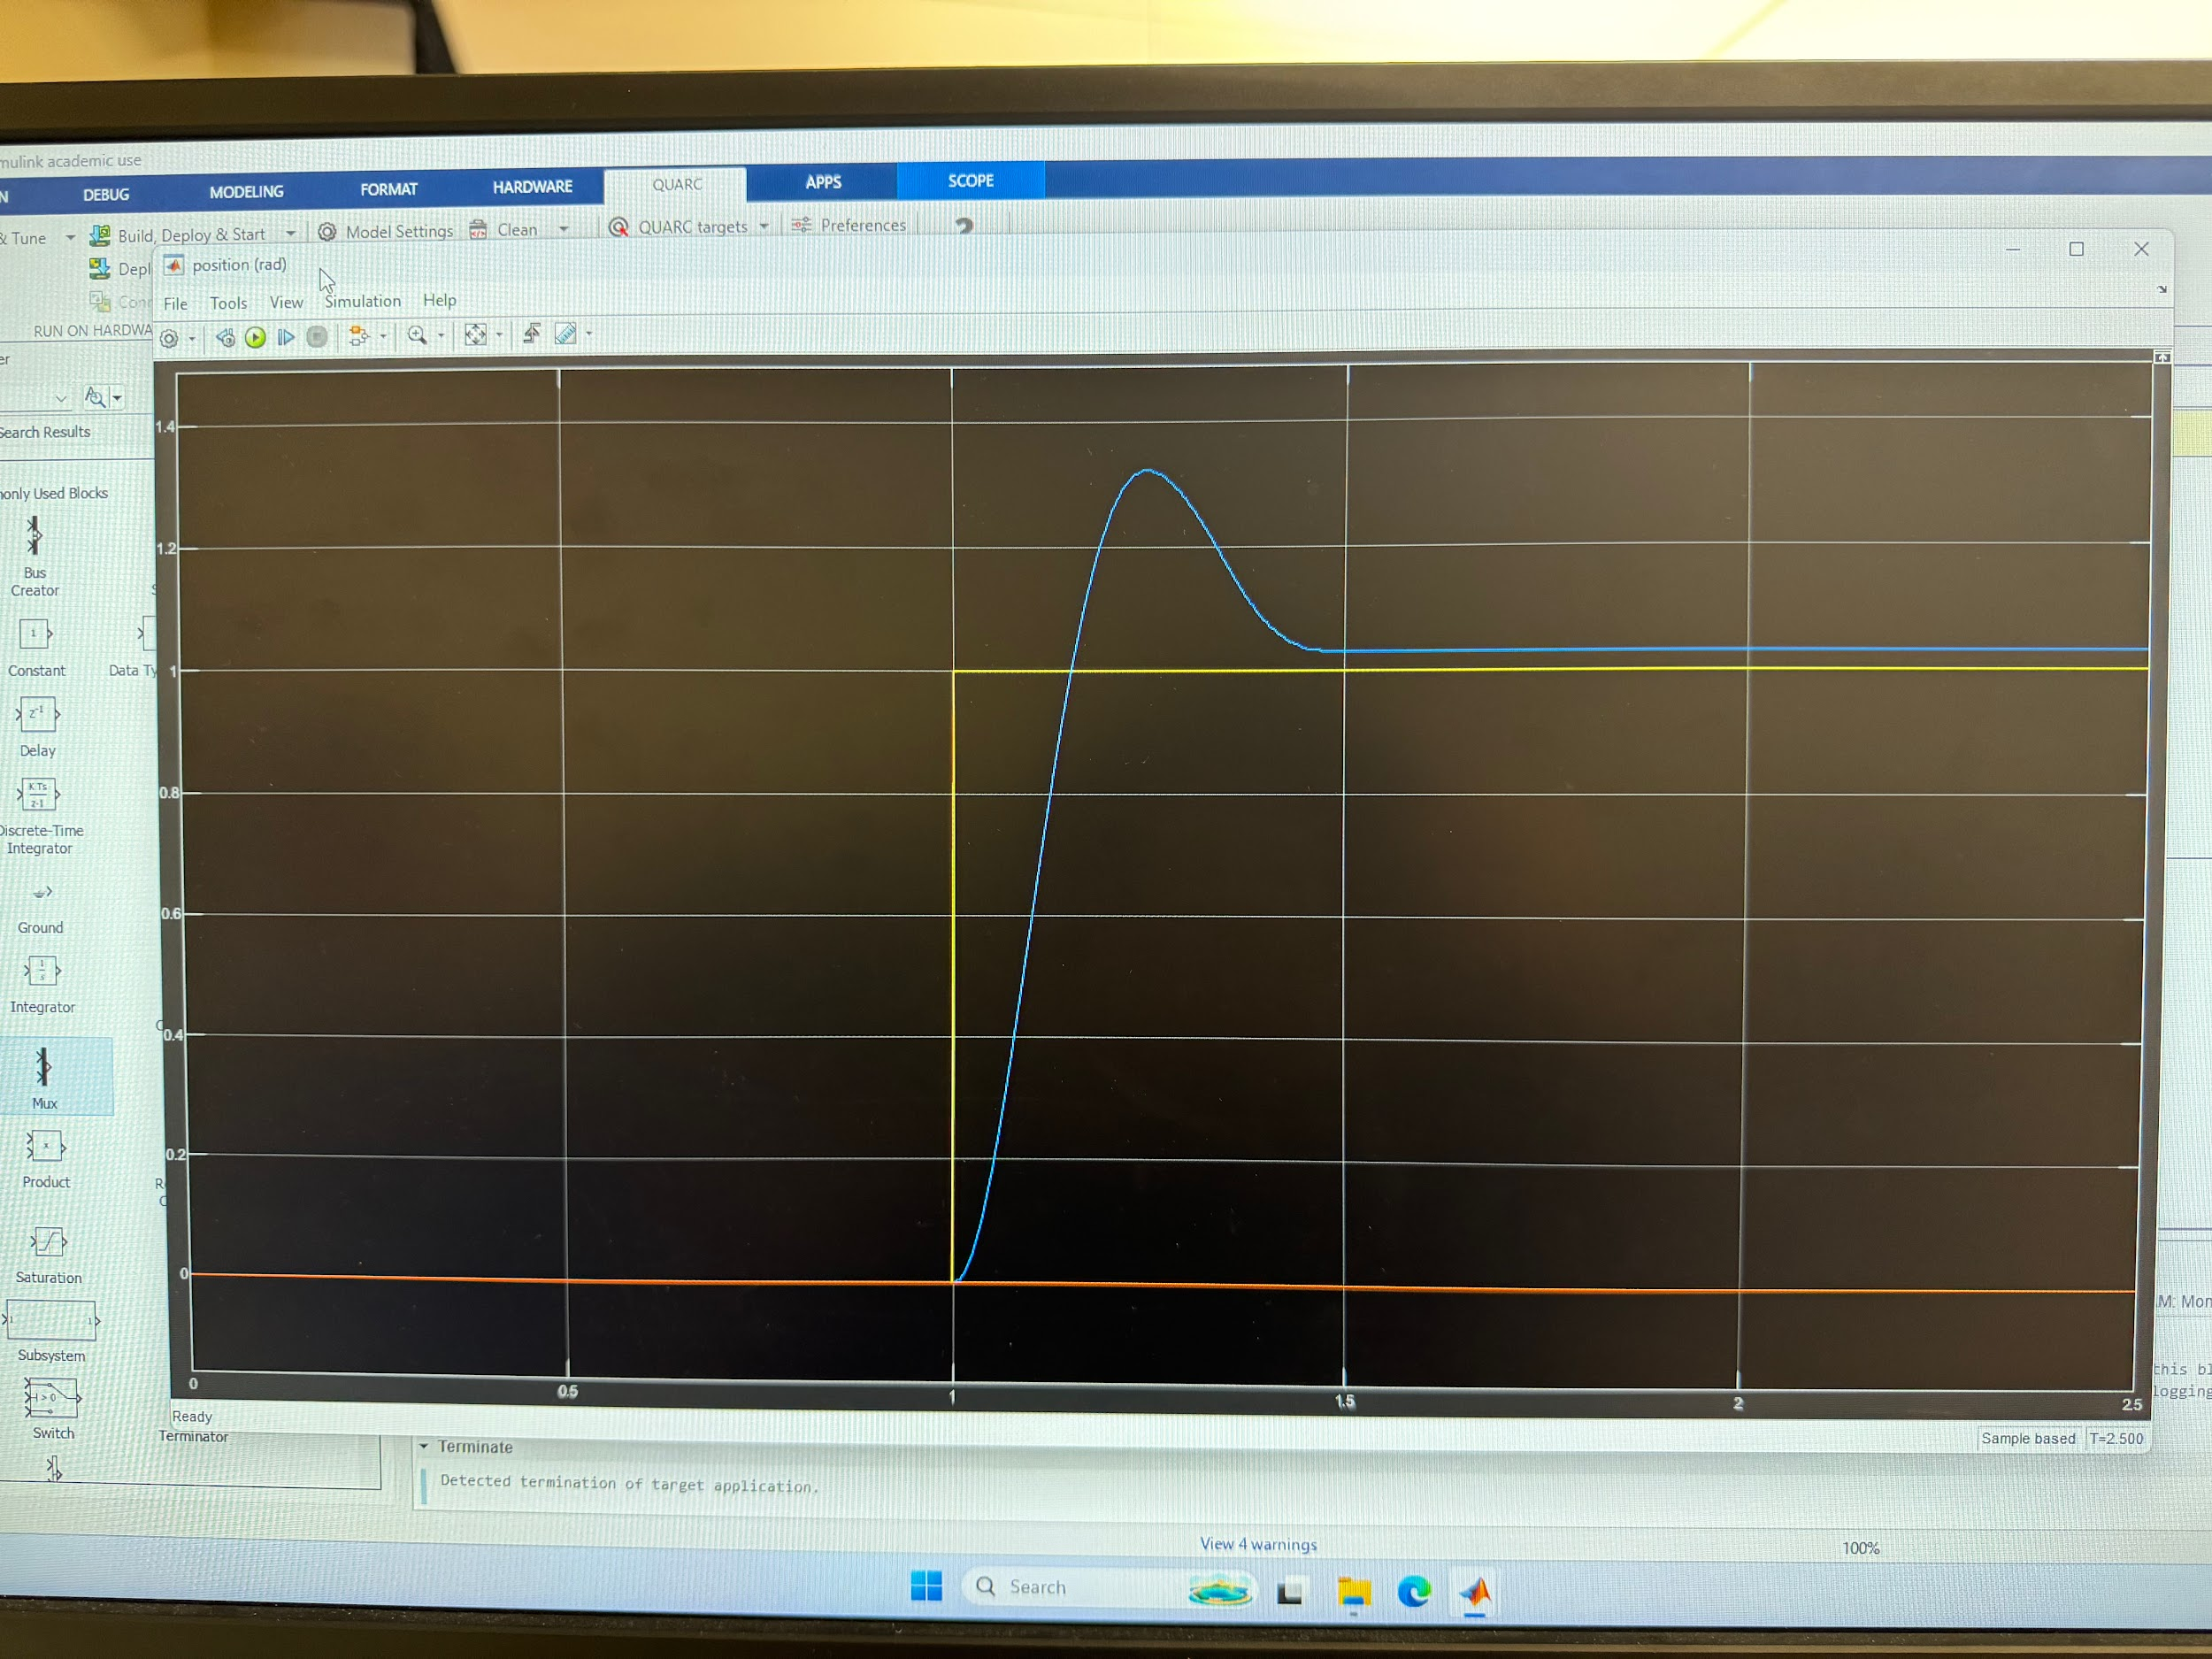
\includegraphics[width=0.88\textwidth]{position.jpg}
    \caption{QUBE-Servo position response. The yellow trace is the \SI{1}{\radian}
    setpoint applied at \SI{1}{\second}; the blue trace is the measured motor position,
    which overshoots before settling, confirming underdamped behavior.}
    \label{fig:position}
\end{figure}

\begin{figure}[H]
    \centering
    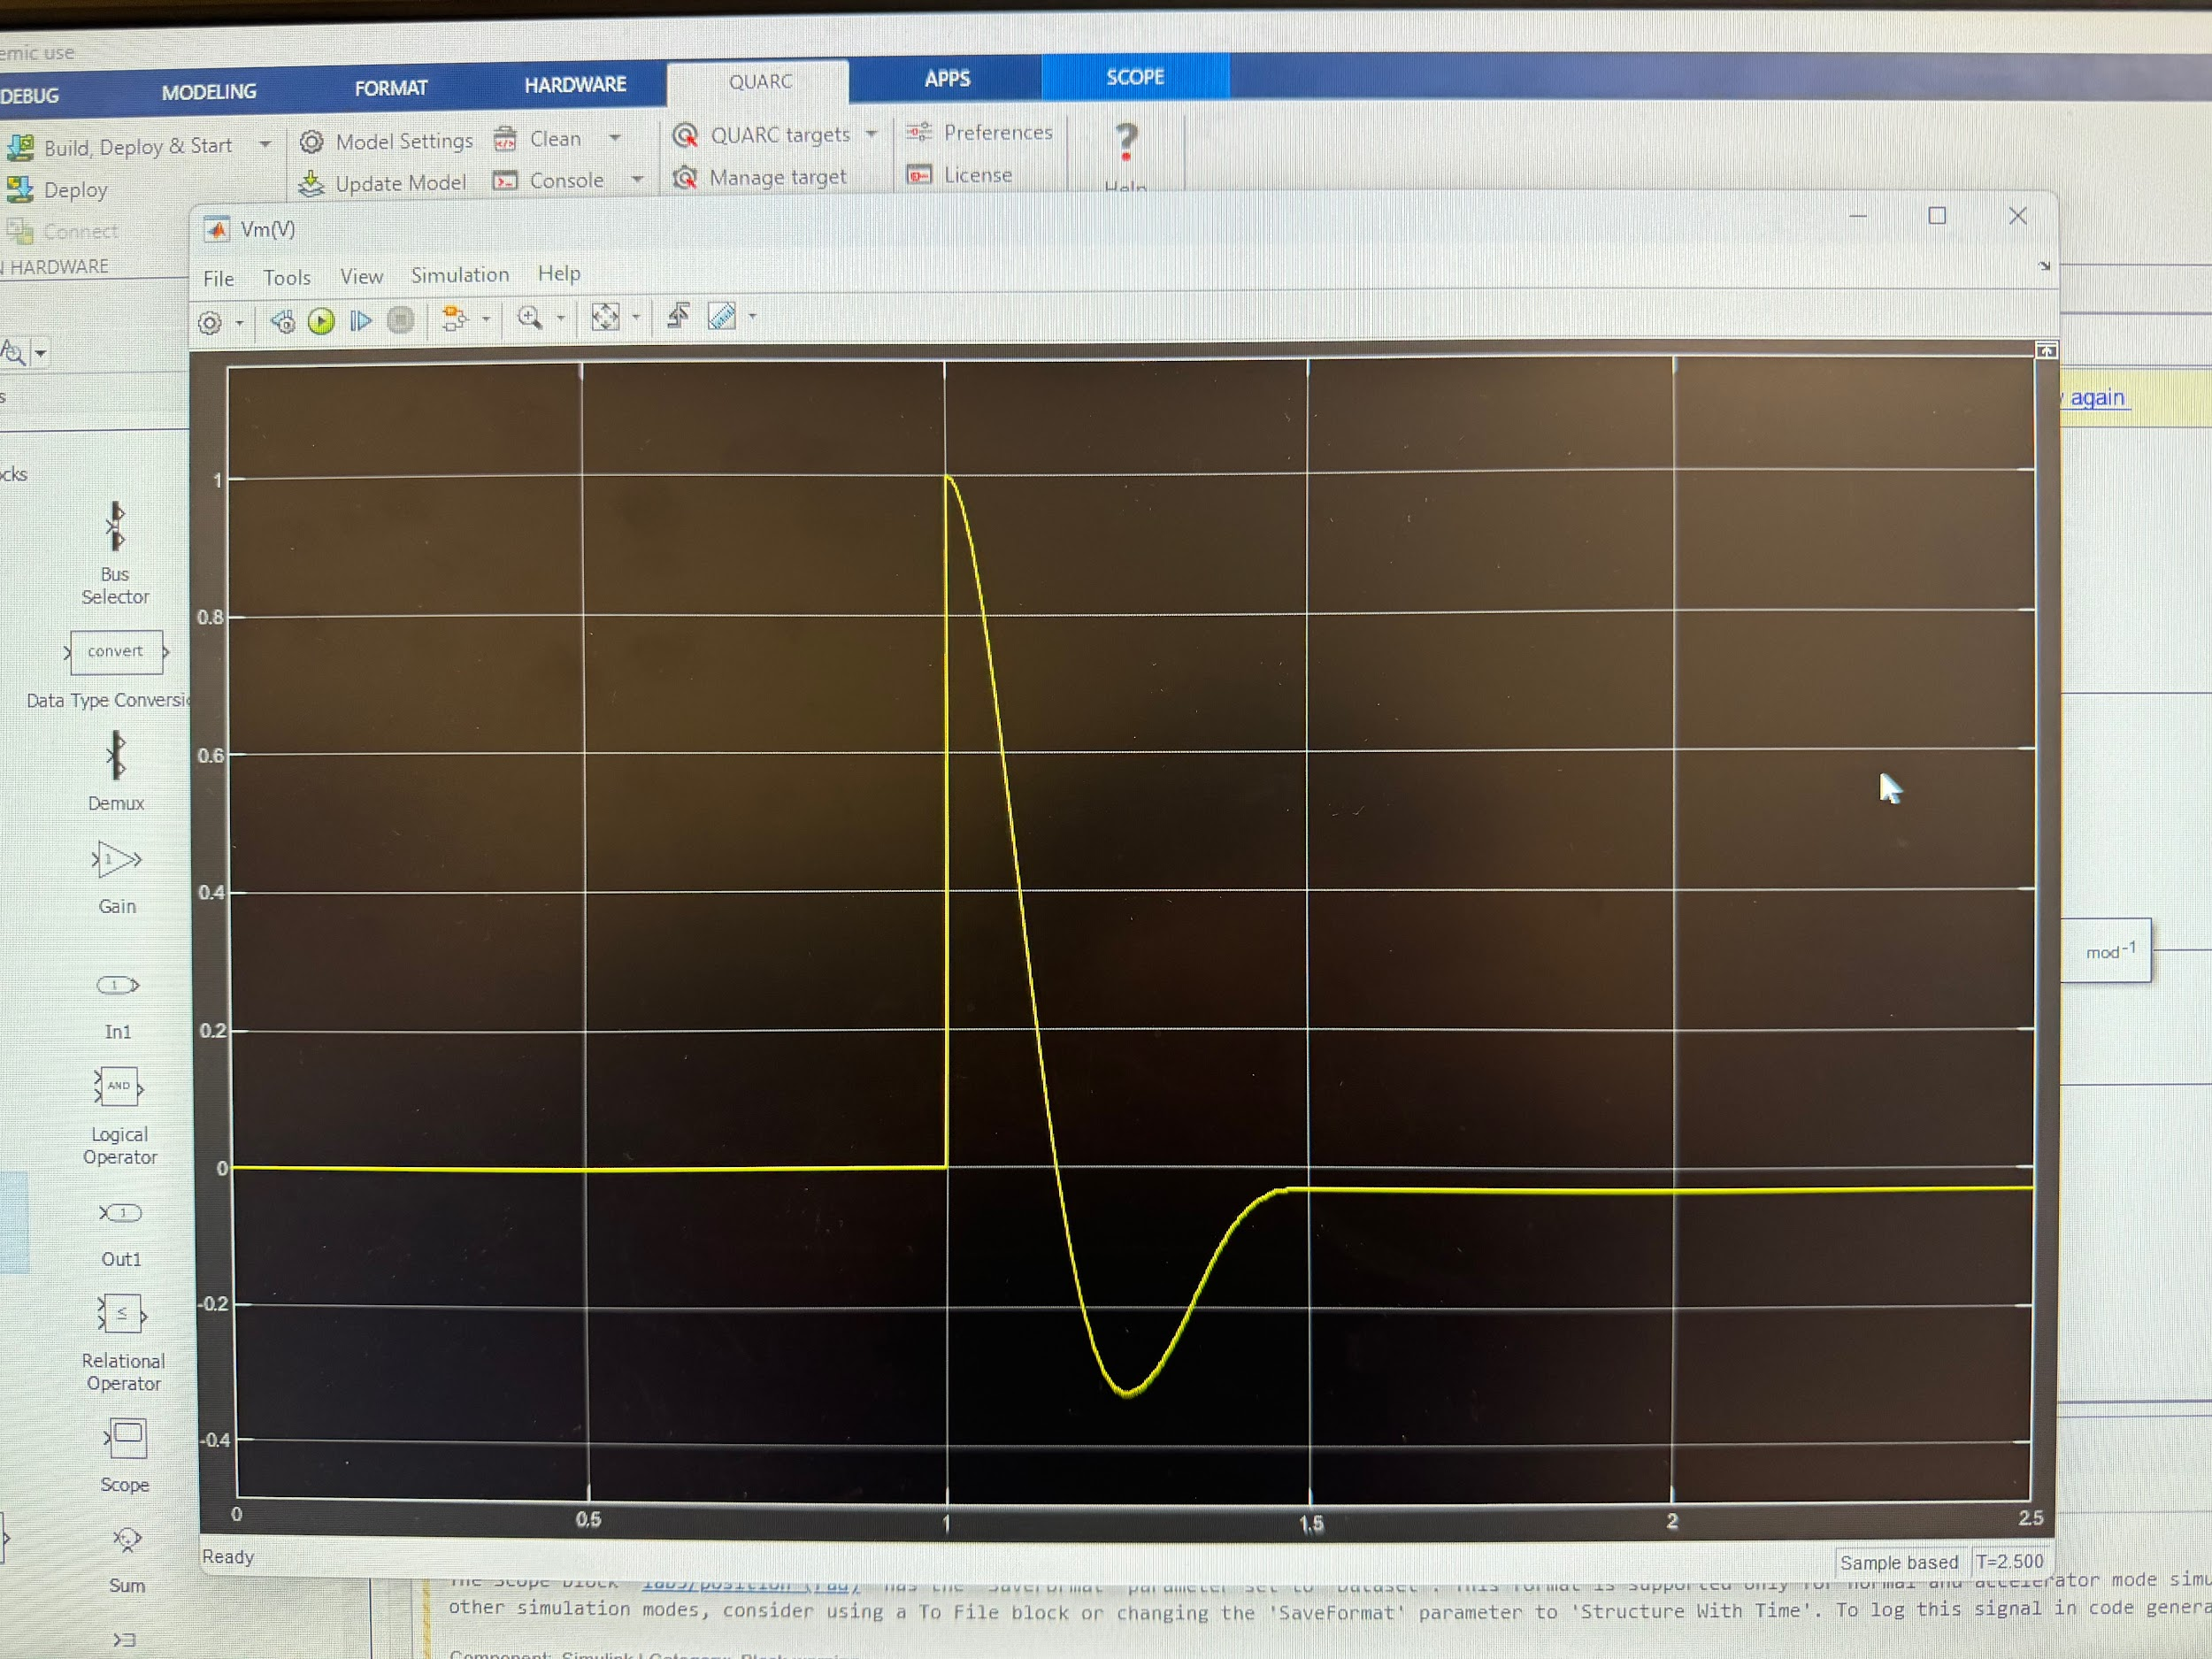
\includegraphics[width=0.88\textwidth]{voltage.jpg}
    \caption{Motor voltage command $V_m$ produced by the unity feedback controller in
    response to the step input.}
    \label{fig:voltage}
\end{figure}

\subsection{Measured Peak Time and Percent Overshoot}
The peak time and percent overshoot were extracted from the logged response using a short
MATLAB script (Figure~\ref{fig:matlab}). The experimental response reached its maximum
value of $y_{\max} = \SI{1.3232}{\radian}$ at $t_{\max} = \SI{1.2380}{\second}$. Since the
step input occurred at $t_0 = \SI{1.0000}{\second}$, the measured peak time was
\begin{equation}
    t_p = t_{\max} - t_0 = \SI{0.2380}{\second},
\end{equation}
and the measured percent overshoot was $\%\mathrm{OS} = 32.2291\%$. These values were close
to the theoretical results, with the experimental peak time slightly faster than expected
and the overshoot within a fraction of a percent of the predicted $32\%$.

\begin{table}[H]
    \centering
    \caption{Comparison of theoretical and measured transient-response metrics.}
    \begin{tabular}{lccc}
        \toprule
        Metric & Theoretical & Measured & \\
        \midrule
        Peak time $t_p$ (\si{\second})     & 0.25 & 0.2380 & \\
        Percent overshoot $\%\mathrm{OS}$  & 32\% & 32.2291\% & \\
        \bottomrule
    \end{tabular}
    \label{tab:compare}
\end{table}

\begin{figure}[H]
    \centering
    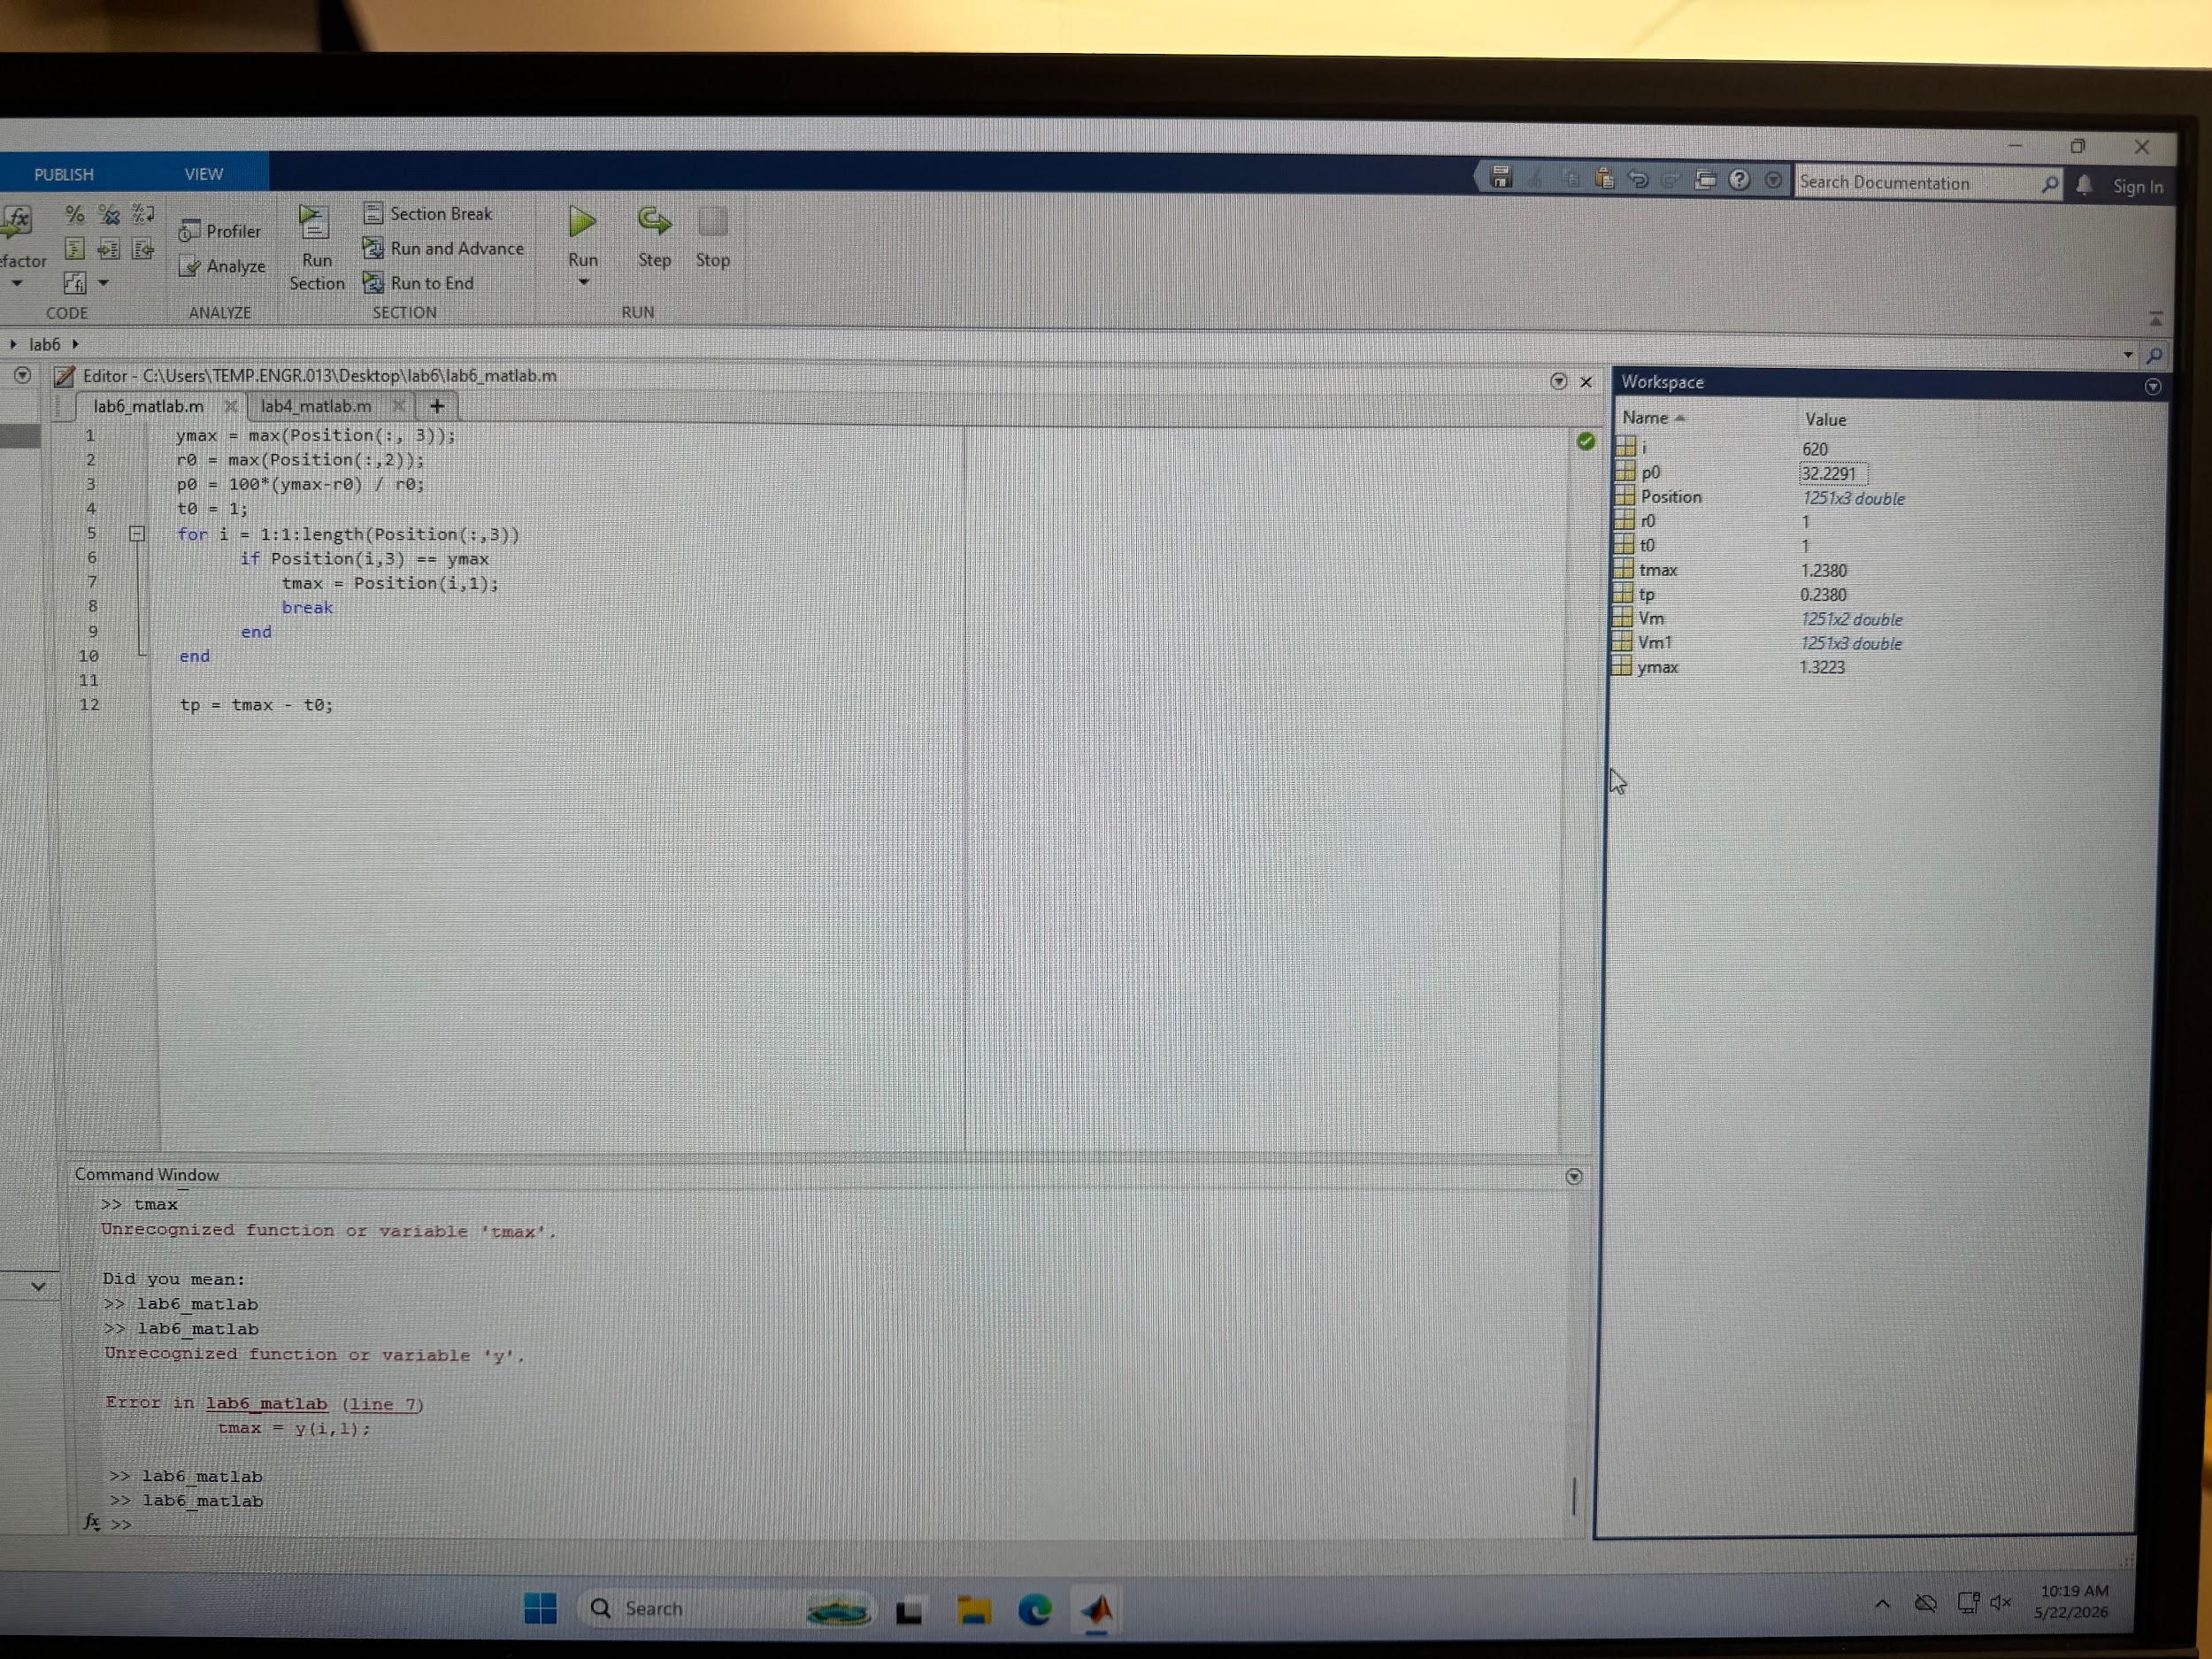
\includegraphics[width=0.92\textwidth]{matlab.jpg}
    \caption{MATLAB script and workspace used to compute the peak value, peak time, and
    percent overshoot from the logged position data
    ($y_{\max}=1.3232$, $t_{\max}=1.2380$, $t_p=0.2380$, $\%\mathrm{OS}=32.2291$).}
    \label{fig:matlab}
\end{figure}

% =====================================================================
\section{Analysis}
% =====================================================================
\textbf{Results analysis.} The results confirmed the expected behavior of an underdamped
second-order system. The QUBE-Servo response showed oscillations and overshoot before
reaching steady state, which aligned with the calculated damping ratio and natural
frequency. The measured peak time and percent overshoot were reasonably close to the
theoretical values, demonstrating that the mathematical model accurately represented the
system dynamics. The experiment also showed how the damping ratio affects the shape of the
response while the natural frequency affects the speed of the response. A lower damping
ratio resulted in larger overshoot and oscillation, while the relatively high natural
frequency allowed the system to respond quickly.

\textbf{Issues encountered.} The only issue encountered was constructing the code. We
worked around it and were able to obtain the correct results.

% =====================================================================
\section{Conclusion}
% =====================================================================
In this lab, a unity feedback position control system was implemented using the Quanser
QUBE-Servo to study second-order system behavior. The experiment successfully demonstrated
concepts such as damping ratio, natural frequency, percent overshoot, and peak time.
Theoretical calculations were compared with experimental measurements, and the results
showed strong agreement between the mathematical model and the physical system response.
Overall, the lab provided practical experience with control systems, Simulink modeling, and
transient response analysis of underdamped second-order systems.

\end{document}
